% ISS presentation template
%
% Change history:
% 24.06.2010    Jürgen Ruoff        Initial creation
% 01.07.2010    Patrick Häcker      Generalization
% 02.07.2010    Patrick Häcker      Adjustment
% 15.11.2010    Patrick Häcker      Improvements
% 20.05.2011    Patrick Häcker      Add presentation type
% 06.01.2012	P. Hermannstädter 	Adapted to ISS, small mods
% \graphicspath{ {../Fig/} }
% Insert your name here
\newcommand{\presenter}{Zhuowei Han}
\newcommand{\presentershort}{Z.Han}
\newcommand{\presenteremail}{} 		% can be accessed using \presenteremail
\newcommand{\x}{\mathbf{x}}
\newcommand{\mX}{\mathbf{X}}
\newcommand{\mH}{\mathbf{H}}
\newcommand{\h}{\mathbf{h}}
\newcommand{\btheta}{\boldsymbol{\theta}}
\newcommand{\y}{\mathbf{y}}
\newcommand{\W}{\mathbf{W}}
\newcommand{\vb}{\mathbf{b}}
\newcommand{\vc}{\mathbf{c}}
\newcommand{\txtcolb}[1]{\textcolor{blue}{\Large #1}}

% Insert presentation title here
\newcommand{\presentationtitle}{Deep Network for Speech Emotion Recognition}
\newcommand{\shortpresentationtitle}{Deep Learning}

% Insert type of presentation here (or comment line), probably one of:
% Mitarbeitervortrag, Bachelor-Arbeit, Master-Arbeit, Bachelor thesis, Master thesis
\newcommand{\presentationtype}{---A Study of Deep Learning---}

% Insert presentation date here
\newcommand{\presentationdate}{16/04/2015}

% Uncomment the following line, if you write in English
%\newcommand{\lang}{german}

% Uncomment the following line, if you want to create handouts (setting to false does not work!)
% \newcommand{\handoutmode}{true}

% Load beamer class using LSS style
% Default \lang to ngerman
\ifx\lang\undefined
	\newcommand{\lang}{ngerman}
\fi

% Set \handout dependant on \handoutmode
\ifx\handoutmode\undefined
	\newcommand{\handout}{}
\else
	\newcommand{\handout}{handout}
\fi

% Make additional colors available
\PassOptionsToPackage{x11names}{xcolor}

% Load the beamer class, set the presentation data and use the LSS layout
\documentclass[\lang,\handout]{beamer}
\author[\presentershort]{\presenter}
\title[\shortpresentationtitle]{\presentationtitle}
\ifx \presentationtype \undefinded
\else
	\subtitle{\presentationtype}
\fi
\date{\presentationdate}
\institute{Institut f�r Signalverarbeitung\\und Systemtheorie\\\vspace{1em}Universit�t Stuttgart}
\usetheme[alternativetitlepage=true,% Use the fancy title page.
          titlepagelogo=isslogocolor,% Logo for the first page.
          watermark=isslogocolor,% Watermark used in every page.
          watermarkheight=25px,% Height of the watermark.
          ]{LSS}

% Grays uncovered objects instead of making them invisible; comment to make uncovered objects invisible
\setbeamercovered{transparent}

% Set work to presentation to not get blue hyperlinks
\newcommand{\work}{presentation}

% Input general definitions and loading of packages which can be shared with the thesis.
% Comment this line if you want to decide yourself which packages should be loaded.
% \def\me{Patrick H�cker}

% this is needed to get more resources to TeX - otherwise not all packages work at the same time
\usepackage{etex}

% erm�glicht ein if-then-else in LaTeX z. B. um Pakete variabel einzubinden
\usepackage{xifthen}
% \newcommand{\ifthen}[1]{\ifthenelse{#1}{}} % It does not work (behaviour is wrong)

% Load language specific things. Always load german, too, to get things like the long name of LSS correctly.
\ifx\lang\undefined
	\newcommand{\lang}{ngerman}
\fi
\ifthenelse{\equal{\lang}{german}}{
	\renewcommand{\lang}{ngerman}
}{}

\ifthenelse{\not\equal{\lang}{ngerman}}{
	\usepackage[ngerman,\lang]{babel}
}{
	\usepackage[\lang]{babel}
}

% damit man Umlaute direkt eingeben kann und diese erkannt werden (sp�ter auf utf8 umsteigen).
\usepackage[x-iso-8859-1]{inputenx}

% Umlaute werden als eine Einheit angesehen -> richtige Trennung und korrekt ins PDF eingebunden;
\usepackage[T1]{fontenc}

% Enth�lt gewisse Sonderzeichen wie z. B. Bullets
\usepackage{textcomp}

% Allow more set symbols (does not replace amsmath symbols if included before amsmath)
\usepackage[bbgreekl]{mathbbol}

% Schaltet AMS-Befehle, Schriftzeichen und Symbole frei (Mathepaket)
% Allow bold uppercase greek letters using the boldsymbol command
\usepackage{amsmath}
\usepackage{amsfonts}
\usepackage{amssymb}

% Allows bold italic uppercase letters
\usepackage{fixmath}



%Erlaubt den Seitenumbruch in Formeln, auch wenn er nach M�glichkeit vermieden wird
\allowdisplaybreaks[4]

% Enables fraction of the form a/b (with a nice slash)
\usepackage{nicefrac}

% Bindet die standardm��ig genutzten Times-Fonts ein (muss nach amsmath eingebunden werden)
% \usepackage{txfonts}

% Uses the Latin Modern font
\usepackage{lmodern}

% erm�glicht die aufrechte Schreibung griechischer Buchstaben
\usepackage{upgreek}

%erm�glicht das Einbinden von EPS-Dateien
\usepackage{graphicx}

%Das nachtr�gliche �ndern von Texten und Anpassen der Schriftart in EPS-Dateien beim Einbinden
\usepackage{psfrag}

%erm�glicht farbigen Text
\usepackage[x11names]{xcolor}

%erm�glicht farbige Tabellenhintergr�nde
\usepackage{colortbl}

% tikz is a cool drawing package using pgf
\usepackage{tikz}

\usetikzlibrary{3d,arrows,automata,backgrounds,calc,calendar,chains,decorations,decorations.footprints,decorations.fractals,decorations.markings,decorations.pathmorphing,decorations.pathreplacing,decorations.shapes,decorations.text,er,fadings,fit,folding,matrix,mindmap,patterns,petri,plothandlers,plotmarks,positioning,scopes,shadows,shapes.arrows,shapes.callouts,shapes,shapes.gates.logic.IEC,shapes.gates.logic.US,shapes.geometric,shapes.misc,shapes.multipart,shapes.symbols,through,topaths,trees}

% pgfplots enables the simple creation of plots from data points (eg. generated by matlab2tikz.m)
\usepackage{pgfplots}

% save every tikz plot as a pdf file (see package documentation of pgfplots)
% \usepgfplotslibrary{external}
% \tikzexternalize{ the main file name }

% If you want to print on a different size, use this package temporally
% \usepackage{pgfpages}
% \pgfpagesuselayout{resize}[a3paper]

% set PGF's decimal separator to comma for german documents
\ifthenelse{\equal{\lang}{ngerman}}{
	\pgfkeys{/pgf/number format/.cd, set decimal separator={{{,}}}}
}{}

% damit kann man Diagramme und Funktionen zeichnen
% \usepackage{pstricks,pst-plot,pst-node}
%\usepackage{pstricks-add}

% Zugriff auf gnuplot aus LaTeX heraus (erfordert -shell-escape bei latex-Aufruf)
% \usepackage{gnuplottex}

%\usepackage{multicol}

% Introduces \vref, a command which adds the page to the reference if necessary
\usepackage{nameref}
\usepackage{varioref}

\ifthenelse{\equal{\work}{thesis} \OR \equal{\work}{paper}}{
	\ifthenelse{\equal{\version}{computer}}{
		\def\colortype{color}
	}{}
	\ifthenelse{\equal{\version}{print}}{
		\def\colortype{black}
	}{}

	% Macht Links und Referenzen farbig und entfernt h�ssliche K�stchen drumherum
	% Hyperlinks blau ('color') (=PC-Version) oder schwarz ('black') (=Druckversion)
	\ifthenelse{\equal{\colortype}{color}}{
		\usepackage[breaklinks=true,colorlinks,linkcolor=blue]{hyperref}
	}{
		\usepackage[breaklinks=true]{hyperref}
	}
}
{
	\usepackage{hyperref}
}

% Makes the boolean ifpdf available to check if LaTeX is directly generating a PDF file


\usepackage{ifpdf}

\ifpdf
\else
	% Sorgt daf�r, dass \url-Befehl automatische Umbr�che unterst�tzt (macht Probleme mit pdflatex)
	\usepackage{breakurl}
\fi

% Erm�glicht Abbildungen, die vom Text umflossen werden
% (zwei unterschiedliche Ans�tze, haben wohl beide Nachteile)
% \usepackage{floatflt}
\usepackage{wrapfig}

% Setzt manche Bildunterschriften n�her ans Bild heran, was sch�ner aussieht
\usepackage[hang]{caption}

% mehrere kleine Tabellen oder Grafiken aneinander anordnen (muss nach caption eingebunden werden)
%\usepackage{subfig}

%\usepackage{subfloat}

% Sauber formatierte Quellcode-Umgebung zur Verf�gung stellen
\usepackage{listings}

% Erm�glicht Tabellen, deren Gesamtbreite eingestellt werden kann, wobei eine Spalte �brigen Platz bekommt
\usepackage{tabularx}

% Erm�glicht Tabellen, deren Gesamtbreite eingestellt werden kann, wobei �briger Platz prozentual aufgeteilt wird
\usepackage{tabulary}

% Erstellt sch�nere Tabellen, wobei vertikale Linien nicht mehr benutzt werden d�rfen
\usepackage{booktabs}

% Erm�glicht Tabellenzellen die Ausdehnung �ber mehrere Zeilen
\usepackage{multirow}

% Writes an additional file to enable backward synchronisation between PDF and LaTeX
% "pdfsync uses extremely sensible code. You should not use pdfsync on final documents because
% it can change the layout rather significantly", yep, I hit a bug
% \usepackage{pdfsync}

% Erm�glicht das hinzuf�gen von fixme-Kommentaren, auch als \todo
\usepackage{fixme}
\newcommand{\todo}[1]{\fxwarning{#1}}
%\usepackage[inline,\status]{fixme}

% Ist f�r die �bergangsphase zu pdflatex sinnvoll, weil dann auch eps-Grafiken eingebunden werden k�nnen
%\usepackage{epstopdf}

% Abk�rzungsverzeichnis erstellen und konfigurieren
%\usepackage[german,intoc]{nomencl}
%\renewcommand{\nomname}{Abk�rzungsverzeichnis}
%\let\abbrev\nomenclature
%\setlength{\nomlabelwidth}{.15\hsize}
%\makenomenclature

% Stellt \doublespacing, \onehalfspacing und \singlespacing zur Verf�gung
\usepackage{setspace}

% Allows putting two images on top of each other
% \usepackage[percent]{overpic}

% The savetrees package packs as much text as possible onto each page
% \usepackage{savetrees}

% Stellt das Kommando \extrarowheight f�r das glossaries-Paket zur Verf�gung
\usepackage{array}

% allows usage of \degree
\usepackage{gensymb}

% Abk�rzungen
% Sets
\newcommand{\Z}{\mathbb{Z}}
\newcommand{\N}{\mathbb{N}}
\newcommand{\Q}{\mathbb{Q}}
\newcommand{\R}{\mathbb{R}}
\newcommand{\C}{\mathbb{C}}

% differentiation
\newcommand{\del}{\partial}
\newcommand{\derivate}[2]{\frac{\del #1}{\del #2}}
\DeclareMathOperator{\dif}{d}
\DeclareMathOperator{\gradlong}{grad}
\DeclareMathOperator{\grad}{\bigtriangledown}

% statistics
\newcommand{\erw}[1]{\operatorname{E}\left(#1\right)}
\DeclareMathOperator{\E}{E}
\DeclareMathOperator{\prop}{P}
\DeclareMathOperator{\Var}{Var}
\DeclareMathOperator{\Cov}{Cov}
\DeclareMathOperator{\Bias}{Bias}
\DeclareMathOperator{\CRB}{CRB}

% linear algebra
\newcommand{\mat}[1]{\mathbf{#1}}
%\newcommand{\mat}[1]{\boldsymbol{#1}}
\newcommand{\Tr}[1]{\mathrm{Tr}\left( #1 \right)} %deprecated
\newcommand{\tr}[1]{\mathrm{tr}\left( #1 \right)}
\newcommand{\rang}[1]{\mathrm{rang}\left( #1 \right)}
\newcommand{\diag}[1]{\mathrm{diag}\left( #1 \right)}
\newcommand{\pinv}[1]{#1^{\dagger}}
\newcommand{\trans}[1]{#1^{\mathrm{T}}}
\newcommand{\hermitian}{\mathrm{H}}
\newcommand{\herm}[1]{#1^\mathrm{H}}
\newcommand{\konj}[1]{#1^{\mathrm{*}}}
\newcommand{\est}[1]{\hat{#1}}
\newcommand{\abs}[1]{\left\lvert#1\right\rvert}
\newcommand{\norm}[1]{\left\lVert#1\right\rVert}

% german abbreviations
\newcommand{\zB}{\mbox{z.\,B. }}
\newcommand{\iA}{\mbox{i.\,A. }}
\newcommand{\deha}{\mbox{d.\,h.\ }}
\newcommand{\oae}{\mbox{o.\,�.\ }}
\newcommand{\uae}{\mbox{u.\,�.\ }}
\newcommand{\oBdA}{\mbox{o.\,B.\,d.\,A. }}
\newcommand{\OBdA}{\mbox{O.\,B.\,d.\,A. }}
\newcommand{\ggf}{\mbox{ggf.\ }}
\newcommand{\vgl}{\mbox{vgl.\ }}
\newcommand{\evtl}{\mbox{evtl.\ }}
\newcommand{\bzw}{\mbox{bzw.\ }}
\newcommand{\bspw}{\mbox{bspw.\ }}
\newcommand{\ca}{\mbox{ca.\ }}

% english abbreviations
\newcommand{\eg}{\mbox{e.g.\ }}
\newcommand{\ie}{\mbox{i.e.\ }}

% quotes
\newcommand{\gq}[1]{\glq#1\grq}
\newcommand{\gqq}[1]{\glqq#1\grqq}
\newcommand{\eq}[1]{`#1'}
\newcommand{\eqq}[1]{``#1''}


% functions
\newcommand{\e}[1]{\operatorname{e}^{\,#1}}
\newcommand{\argmax}[2]{\underset{#1}{\operatorname{argmax}}\left( #2 \right)}
\newcommand{\argmaxima}[2]{\underset{#1}{\operatorname{argmaxima}}\left( #2 \right)}
\newcommand{\argmin}[2]{\underset{#1}{\operatorname{argmin}}\left( #2 \right)}
\DeclareMathOperator{\arc}{arc}
\DeclareMathOperator{\sinc}{sinc}
\DeclareMathOperator{\ggT}{ggT}
\DeclareMathOperator{\kgV}{kgV}
\DeclareMathOperator{\lcm}{lcm}

% symbols
% \newcommand{\degree}{\ensuremath{^\circ}}
\newcommand{\entspricht}{\mathrel{\hat{=}}}
\newcommand{\sollgleich}[0]{\overset{!}{=}}
\newcommand{\help}{\textcircled{\scriptsize{?}}}

% general
\newcommand{\op}[1]{\operatorname{#1}}
\newcommand{\smtext}[1]{{\scriptscriptstyle\text{#1}}}
%Zeilenumbruch mit eineinhalbzeiligem Abstand
\newcommand{\br}{\vspace{0.6em}\newline} %entspricht etwa \par\smallskip, geht aber auch in captions
\newcommand{\unit}[2]{\ensuremath{#1}\,\ensuremath{\mathrm{#2}}}
% \newcommand{\definition}[1]{\textit{#1}}
\newcommand{\includeplot}[1]{\centering\includegraphics{parent/Plots/#1.eps}}
\newcommand{\link}[1]{\href{#1}{\url{#1}}}
\newcommand{\shortlink}[1]{\href{#1}{#1}}
\newcommand{\mailto}[1]{\href{mailto:#1}{#1}}
\newcommand{\textlink}[2]{\href{#2}{\url{#1}}}
\newcommand{\vecfun}[2]{#1\hspace{-0.1em}\left(\vec #2\right)}
\newcommand{\equal}[1]{\overset{\text{#1}}{=}}
\newcommand{\matlab}{\textsc{Matlab}\raisebox{1ex}{\tiny{\textregistered}} }

% renews
\renewcommand{\inf}{\infty}
\renewcommand{\matrix}[1]{\mathbf{#1}}
\renewcommand{\j}{\mathrm{j}}
\renewcommand{\gcd}[0]{\operatorname{gcd}}
\renewcommand{\-}{\,--\,}


% Definiert den Befehl \writetofile, der als erstes Argument den Dateinamen und als zweiten Befehl den zu schreibenden Text erwartet
\newcommand{\writetofile}[2]{
% Erstelle Variable outfile
\newwrite\outfile
%�ffne Datei mit Handle outfile
 \immediate\openout\outfile=#1
%Schreibe in Datei
 \immediate\write\outfile{#2}
%Schlie�e Datei
\immediate\closeout\outfile
}

\newcommand{\readfromfile}[1]{
\newread\infile
\immediate\openin\infile=#1
\immediate\read\infile to \tempXBE
\immediate\closein\infile
\tempXBE
}


% \newcommand{\dotsnewline}{\mydotfill\,\linebreak.}

% Allgemeinerer Ansatz als Paket nomencl um mehrere Abk�rzungs-/Symbolverzeichnisse zu erstellen
% Glossary "acronym" wird vordefiniert und Glorraries kommen in Inhaltsverzeichnis (toc)
% einsetzbar: toclike2, toclike3
%\usepackage[acronym,toc,style=toclike3acronym]{glossaries}
% deactivate toclike3acronym temporally due to squeeze upgrade

% Deactivated here and activated in main document, as makeglossaries does not work otherwise (WTF?)
% \usepackage[acronym,toc,style=listdotted]{glossaries}

% Abschlie�ender Punkt in jeder Zeile wird weggelassen
% \renewcommand{\glspostdescription}{}
% L�sst Leerzeile bei Anfangsbuchstabenwechsel in den Verzeichnissen weg
% \renewcommand{\glsgroupskip}{}

% \newcommand{\newacronymdots}[2]{\newglossaryentry{#1}{type=\acronymtype, name={#1}, description={#2}, text={#1}, first={#2 (#1)}, plural={#1s}, firstplural={#2s (#1s)}, symbol={\dotsnewline}}}


% \newcount\boolcounter
% \boolcounter=1
% \advance\boolcounter by 1
% erm�gliche Kennzeichnung eines Akronyms im Text durch \acronym{was}
%%%\newcommand{\acronym}[1]{\acr{#1}}
% \newcommand{\acronym}[1]{\gls{#1}}
% \let\acronym\gls
% \newcommand{\acronym}[1]{#1}
%\newcommand{\acronymnolink}[1]{\protect\acr*{#1}}
% erm�glicht die Benutzung eins Akronyms mit beliebigem Text (Argument #2)
% \newcommand{\acronymtext}[2]{\glslink{#1}{#2}}
% erm�glicht das Benutzen eines Akronyms, ohne dass die ausgeschriebene Version (dieses Mal) verwendet wird
% \newcommand{\acronymshort}[1]{\glslink{#1}{#1}}
% Verwendet ein Akronym ohne einen Link zu setzen (geht nicht in floating-Umgebungen)
%\newcommand{\acronymnolink}[1]{#1\glsadd{#1}}
% erm�gliche Definition eines Akronyms in akronyme.tex durch \defineacronym{was}{wie}
% \newcommand{\defineacronym}[2]{\newacronym{#1}{#1}{#2}}
% \newcommand{\defineacronym}[2]{}
% \newcommand{\defineacronymdots}[2]{\newacronymdots{#1}{#2}}
%Sorgt daf�r, dass man "\acronym{DoS}[-Angriff]" schreiben kann und dann automatisch "DoS-Angriff (Denial of Service)"
%geschrieben wird, bzw. "DoS-Angriff", je nachdem, ob es das erste Mal ist oder nicht
% \defglsdisplayfirst[acronym]{#3#4 (#2)}
% analog zu Akronymen: \definevar legt Symbol an, \var referenziert dieses
% \let\var\gls
% \newcommand{\var}[1]{#1}
% \newcommand{\var}[1]{\ifodd\boolcounter{%
% \protect\gls*{#1}%
% }\else%
% \text{\gls{#1}}\fi%
% }
%\newcommand{\varshort}[1]{\text{\glslink{#1}}\text{#1}}
%\newcommand{\varquiet}[1]{\glsadd{#1}}
%\newcommand{\definevar}[3]{\newglossaryentry{#1}{name=\ensuremath{#2},description={#3},sort=#1}}
\newcommand{\definevar}[4]{\newglossaryentry{#2}{name=\ensuremath{#3},description={#4},sort=#1}}
% \newcommand{\definevar}[4]{}
%\newcount\varcounter
%\varcounter=1
%\newcommand{\definevar}[3]{\definevariable{#1}{#2}{\arabic\varcounter #3}{\arabic\varcounter}}%{\arabic\varcounter}\advance\varcounter by 1}
%\newcommand{\definevariable}[4]{\newglossaryentry{#1}{name=\ensuremath{#2},description={#3},sort={#4}}\advance\varcounter by 1}
%\newcommand{\definevar}[4][\DefaultOpt]{%
%\def\DefaultOpt{#2}%
%\newglossaryentry{#2}{name=\ensuremath{#3},description={#1 wird sortiert #4},sort=#1}%
%\newglossaryentry{#2}{name=\ensuremath{#3},description={#4}}%
%}
% \newcommand{\varnolink}[1]{\protect\gls*{#1}}

% create glossaries internally (deactivated here, as this results in an error, must be activated in main file (WTF?))
% \makeglossaries

% \let\addtocontentsOld\addtocontents
% \renewcommand{\addtocontents}[2]{\advance\boolcounter by 1 \addtocontentsOld{#1}{#2} \advance\boolcounter by 1}

%Problem: Hochzahlen sitzen um Variablen mit Index unsauber, tempor�re L�sung:
%\text{\glslink{thetaHatDNF}{$\hat{\vec{\theta}}_{\mathrm{DNF}}^3$}}
%anstatt:
%\var{thetaHatDNF}^3

% unknown hyphenation rules
\hyphenation{Im-puls-ant-wort Im-puls-ant-wort-ko-ef-fi-zien-ten
Pro-gramm-aus-schnitt Mi-kro-fon-sig-nal Sig-nal Rech-ner-ar-chi-tek-tur
Rech-ner-ar-chi-tek-tur-en Leucht-dich-te-mess-ka-me-ra Gam-ma-kor-rek-tur IEEE
Grund-an-nah-me}

% Definiert die Farbe Gray aus gray mit 80% S�ttigung
\definecolor{Gray}{gray}{0.8}

%definiert deutsche hyperref-Bezeichner so um, dass \autoref problemlos funktioniert
% \ifthenelse{\equal{\lang}{ngerman}}{
% 	\addto\extrasngerman{%
% 		\def\appendixautorefname{Anhang}%
% 		\def\chapterautorefname{Kapitel}%
% 		\def\equationautorefname{Gleichung}%
% 		\def\itemautorefname{Punkt}%
% 		\def\pageautorefname{Seite}%
% 		\def\partautorefname{Teil}%
% 		\def\sectionautorefname{Kapitel}%
% 		\def\subsectionautorefname{Kapitel}%
% 		\def\figureautorefname{Abbildung}%
% 		\def\footnoteautorefname{Fu�note}%
% 		\def\tableautorefname{Tabelle}%
% 	}
% }{
% 	\addto\extrasngerman{%
% 		\def\appendixautorefname{Appendix}%
% 		\def\chapterautorefname{Chapter}%
% 		\def\equationautorefname{Equation}%
% 		\def\itemautorefname{Item}%
% 		\def\pageautorefname{Page}%
% 		\def\partautorefname{Part}%
% 		\def\sectionautorefname{Chapter}%
% 		\def\subsectionautorefname{Chapter}%
% 		\def\figureautorefname{Figure}%
% 		\def\footnoteautorefname{Footnote}%
% 		\def\tableautorefname{Table}%
% 	}
% }


% define autoref to act like eqref for equations
\makeatletter
\@ifdefinable\equationname{%
\let\equationname\equationautorefname%
}
\addto\extrasenglish{%
\def\equationautorefname~#1\@empty\@empty\null{(#1\@empty\@empty\null)}
}
% \addto\extrasngerman{%
% \def\equationautorefname~#1\@empty\@empty\null{\equationname~(#1\@empty\@empty\null)}
% }
\makeatother

% Use serifs in math environment and no serifs in text environment
\usefonttheme[onlymath]{serif}

% Define two practical lengths, which can be uses when setting the size of graphics
\newlength\fullwidth
\setlength\fullwidth{11cm}
\newlength\fullheight
\setlength\fullheight{6.8cm}

% Set lines a bit thicker in presentations when using pgfplots to allow recognition of colored lines
\ifx\pgfplotsset\undefined
	%
\else
	\pgfplotsset{every axis/.append style={thick}}
\fi

% Put four slides on each page if handout mode activated
\ifx\handoutmode\undefined
	%
\else
	\usepackage{pgfpages}
	\pgfpagesuselayout{4 on 1}[a4paper,border shrink=5mm,landscape]
	% use this line instead, if you have problems with rotated eps files
	% \pgfpagesuselayout{4 on 1}[border shrink=5mm,landscape]
\fi


% Define Layout parameters:
\setlength{\itemsep}{0.5em}


\usepackage{setspace}
\usepackage{graphicx}
\usepackage{amsmath}
\usepackage{pgfpages}
\usepackage{subfigure}
\usepackage{colortbl}
\graphicspath{ {../Fig/} }
\usepackage[beamer]{hf-tikz}
\usepackage{tikz}
% \setbeameroption{show notes on second screen=left}
% \setbeameroption{second mode text on second screen=left}
% \setbeameroption{show notes}
% \setbeameroption{show notes on second screen=left}


% My commands:

% -----------------------------------------------------------------------------
% -----------------------------------------------------------------------------
\begin{document}
\lstset{basicstyle=\small\ttfamily,xleftmargin=15pt,language=Matlab,
        commentstyle=\color{green},showstringspaces=false,stringstyle=\color{magenta}\ttfamily}

% -----------------------------------------------------------------------------
% This is the title page
\begin{frame}[t,plain]
	\titlepage
\end{frame}


% -----------------------------------------------------------------------------
% Motivation slide
\begin{frame}[t]{Motivation} % 1 folie
% \textcolor{blue}{\Large Training objective}
\only<1-1>{
\textcolor{blue}{\Large Speech Emotion Recognition}\\
	\begin{itemize}
		\itemsep20pt
		\item Most current work focuses on speech processing based on linguistic information,  e.g.: Skype Translator
		\item More natural human-machine interaction requires paralinguistic information such as age, gender, emotion.
		\item Speech Recognition / Speeker Identification / Emotion Recognition
		\only<1-1>{\begin{figure}[b]
		 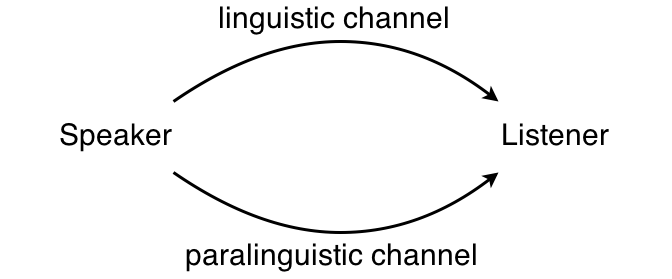
\includegraphics[width=0.6\linewidth]{paraliguistic.png}
		\end{figure}}

	\end{itemize}
}

\only<2-2>{
\textcolor{blue}{\Large Deep Learning}\\
	\begin{itemize}
	    \itemsep15pt
	    \item Deep architecture for extracting complex structure and building internal representations from input
	    \item New research area of machine learning (from shallow to deep structure)
	    \item Widely applied in vision/audition processing, e.g. handwriting recognition (Graves, Alex, et al. 2009), traffic sign classification (Schmidhuber, et al. 2011), text translation (Google, 2014)
	\end{itemize}
}
\end{frame}

% -----------------------------------------------------------------------------
% This is the table of contents. You can insert a motivation before or after this slide.
\begin{frame}
	\ifthenelse{\equal{\lang}{ngerman}}{
		\frametitle{Table of Contents}
	}{
		\frametitle{Table of Contents}
	}
	\tableofcontents
\end{frame}

% Add an extra slide at the beginning of each section while highlighting the current section
% Use \section* to skip the slide once or comment the following to skip all overview slides.
\AtBeginSection[]
{
	\begin{frame}<beamer>
		\ifthenelse{\equal{\lang}{ngerman}}{
			\frametitle{Table of Contents}
		}{
			\frametitle{Table of Contents}
		}
% 		\frametitle{\contentsname}
		\tableofcontents[currentsection]
	\end{frame}
}

%% =========
\section{Foundations} %2 folies
% -----------------------------------------------------------------------------
\subsection{Mel Frequency Cepstral Features}
	\begin{frame}[t]{Mel Frequency Cepstral Features}
		\begin{minipage}[t]{0.48\linewidth}
			\begin{itemize}
				\item short-term power spectrum 
				\item mel-scale approximate human perception
				\item widely-used in speech recognition tasks
				\item Transformation between Mel and Hertz scale
				\begin{figure}

				\begin{eqnarray}
				f_{mel} = 1125~\ln~(1+f_{Hz}/700)\nonumber\\
				f_{Hz} = 700 \left(\exp(f_{mel}/1125)-1\right)\nonumber
				\end{eqnarray}

			\end{figure}
			\end{itemize}
		\end{minipage}
		\begin{minipage}[t]{0.48\linewidth}
		\begin{figure}
		 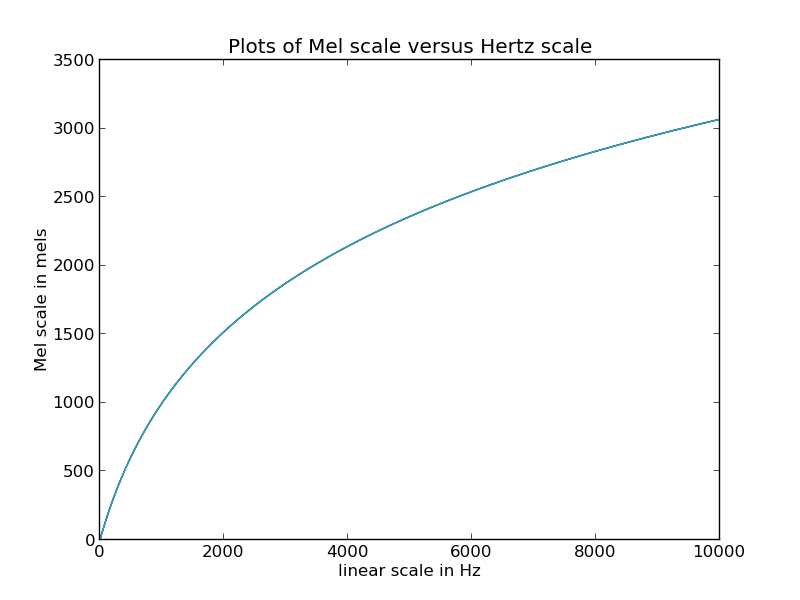
\includegraphics[width = \linewidth]{MelvsHz.png}
		\end{figure}
		\end{minipage}
	\end{frame}


\subsection{Emotion Recognition Approaches}

\begin{frame}[t]{Emotion Recognition Approaches}
	\begin{minipage}[t]{0.48\linewidth}
	  \textcolor{blue}{\Large Traditional Approaches}
	  \begin{itemize}
	   \item pre-selected features
	   \item supervised training
	   \item low-level features not appropriate for claasification
	   \item shallow structure of classifiers
	  \end{itemize}
	\end{minipage}\hfill
	\begin{minipage}[t]{0.48\linewidth}
	\textcolor{blue}{\Large Deep Learning Approaches}
	  \begin{itemize}
	   \item learning representations from high-dim data
	   \item extracting appropriate features without hand-crafting
	   \item low-level features are used to build high-level features as network gets deeper
	   \item frame-based classification
	  \end{itemize}

	\end{minipage}

\end{frame}


\section{Conditional Restricted Boltzmann Machine} %% 



    \subsection{Restricted Boltzmann Machine}
	\begin{frame}[t]{Concepts}
% 	\txtcolb{}
	 \begin{itemize}
	  \itemsep10pt
	  \item Generative graphical model, capture data distrbution $P(\x|\boldsymbol{\theta})$
	  \item Trained in unsupervised way, only use unlabeled input sequence$\x$ for learning. 
		  \begin{itemize}
		   \item automatically extract useful features from data 
		   \item Find hidden structure (distribution). 
		   \item Learned features used for prediction or classification
		  \end{itemize}
	  \item Successfully applied in motion capture (Graham W. Taylor, Geoffrey E. Hinton, 2006)
% 	  \item speicifies a joint distribution over input and hidden variables, can either generating data, or with bayesian
% rule to form conditional distribution. 
	  \item Potential to be extend to capture temporal information
	 \end{itemize}


	
% 	\begin{minipage}[t]{\linewidth}
% 	 $\x$, input units\\
% 	 $\h$, hidden units
% 	\end{minipage}

	\end{frame}
	
	\begin{frame}[t]{Restricted Boltzmann Machine}
	\txtcolb{Structure}
	    \begin{figure}[t]
	    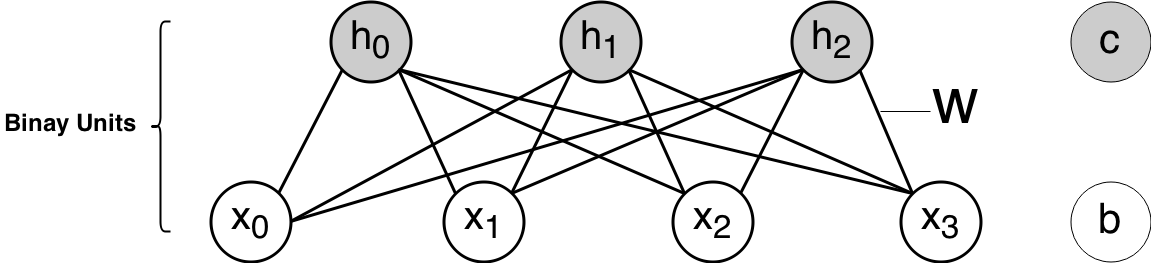
\includegraphics[width=0.9\linewidth]{RBMStruct.png}
	    \end{figure}
	    \only<2->{
	    \begin{minipage}{0.48\linewidth}
	    \begin{align}
	      \text{Energy Function:}~&E_{\boldsymbol{\theta}} = -\mathbf{x^{T}}\mathbf{W}\mathbf{h}-\mathbf{b^{T}}\mathbf{x}-\mathbf{c^{T}}\mathbf{h}\nonumber\\
	    \text{Joint Distribution:}~&P^{RBM} (\mathbf{x},\mathbf{h}) = \frac{1}{Z} e^{-E_{\boldsymbol{\theta}}(\mathbf{x},\mathbf{h})}\nonumber\\
	     \text{Partition Function:}~ &Z = \sum_{\mathbf{x,h}} e^{-E_{\boldsymbol{\theta}}(\mathbf{x},\mathbf{h})}\nonumber\\
	     \text{Free Energy:}~& \mathcal{F}(\mathbf{x}) = - \log \sum_h e^{-E(\mathbf{x,h})}\nonumber
	    \end{align}
	    \end{minipage}
	    }
	\end{frame}
	
	\begin{frame}[t]{Inference}
	\txtcolb{Inference}
		\begin{minipage}[t]{0.48\linewidth}
% 		\begin{figure}[t]
			 \begin{align}
			 &P(\mathbf{x}) = \sum_{\mathbf{h}} P(\mathbf{x,h})\nonumber\\ 
			 &P (\mathbf{h}) = \sum_{\mathbf{x}} P(\mathbf{x,h})\nonumber\\
			 \only<2->{&P (\h|\x)= \dfrac{P(\x,\h)}{P(\x)}\nonumber\\
			 &P(\x|\h)= \dfrac{P(\x,\h)}{P(\h)}\nonumber\\}
			 \only<3->{&P(h_{j}=1 \mid \mathbf{x})= sigmoid(\sum_{i} x_{i}W_{ij} + c_{j})\nonumber\\
			 &P(x_{i}=1 \mid \mathbf{h}) = sigmoid(\sum_{j} W_{ij} h_{j} + b_{i})\nonumber}
			 \notag
			 \end{align}
% 		\end{figure}
	\end{minipage}
% 	\begin{minipage}{0.48\linewidth}
% % 		\begin{figure}[t]
% 			\begin{eqnarray}
% 			\end{eqnarray}
% % 		\end{figure}
% 	\end{minipage}

	\vspace{5mm}
	 
	\end{frame}
 \subsection{CRBM}
	\begin{frame}[t]{Conditional RBM}
	    \only<1-2>{
	    \begin{itemize}
	     \item Consider visible units from previous time step as additional bias for current visible and hidden layer
	     \item $A$ and $B$ are weight parameter of visible (history) - visible and visible (history) - hidden connections
	     \item Visible layer is linear units with independent Gaussian noise to model real-valued data, e.g. spectral features
	    \end{itemize}
	    }
	    \only<2->{
	    \begin{figure}[t]
	    \includegraphics<2>[width=0.7\linewidth]{CRBM.png}
	    \includegraphics<3>[scale = 0.2]{CRBM.png}
	    \end{figure}
	    }
	    \only<3->{\begin{align}
	      \text{Energy Function:}~&E^{CRBM}_{\boldsymbol{\theta}} (\mathbf{x}, \mathbf{h})  = \left\| \frac{\mathbf{x} - \tilde{\mathbf{b}}}{2} \right\|^{2}
    -\tilde{\mathbf{c}}^T \mathbf{h}-\mathbf{x}^{T} \mathbf{W}\mathbf{h} \nonumber\\
	      &\tilde{\mathbf{b}} = \mathbf{b} + \mathbf{A}\cdot \mathbf{x}_{<t}\nonumber\\
	      &\tilde{\mathbf{c}} = \mathbf{c} + \mathbf{B}\cdot \mathbf{x}_{<t}\nonumber\\
	      &\boldsymbol{\theta} = \left \{\mathbf{W,A,B,b,c} \right\}\nonumber\\
	      \text{Free Energy:}~&\mathcal{F}(\mathbf{x}) = \left\| \mathbf{x} - \tilde{\mathbf{b}} \right\|^{2} - \log (1+e^{\tilde{\mathbf{c}}+\mathbf{x}\cdot \mathbf{W}})\nonumber
	    \end{align}
	    }


	\end{frame}
	
	\begin{frame}[t]{Conditional RBM}
	      \begin{align}
		\text{Energy Function:}~&E^{CRBM}_{\boldsymbol{\theta}} (\mathbf{x}, \mathbf{h})  = \left\| \frac{\mathbf{x} - \tilde{\mathbf{b}}}{2} \right\|^{2}
      -\tilde{\mathbf{c}}^T \mathbf{h}-\mathbf{x}^{T} \mathbf{W}\mathbf{h} \nonumber\\
		\text{Free Energy:}~&\mathcal{F}(\mathbf{x}) = \left\| \mathbf{x} - \tilde{\mathbf{b}} \right\|^{2} - \log (1+e^{\tilde{\mathbf{c}}+\mathbf{x}\cdot \mathbf{W}})\nonumber\\
		&\tilde{\mathbf{b}} = \mathbf{b} + \mathbf{A}\cdot \mathbf{x}_{<t}\nonumber\\
		&\tilde{\mathbf{c}} = \mathbf{c} + \mathbf{B}\cdot \mathbf{x}_{<t}\nonumber\\
		&\boldsymbol{\theta} = \left \{\mathbf{W,A,B,b,c} \right\}\nonumber
	      \end{align}
	\end{frame}
	
	\begin{frame}[t]{Training of Energy-based Model}
	      \begin{columns}[c]
		    \column{3in}
		    \alert<1-1>{Maximum Likelihood Estimation} $P(\x|\btheta)$\vspace{5mm}
		    \only<2->{
		    \textcolor{blue}{Kullback-Leibler Divergence}:\\
		    \begin{align}
			KL(Q(\x)\|P(\x|\btheta)) &=  \int_{-\infty}^{\infty} Q(\x)\cdot \log \dfrac{Q(\x)}{P(\x|\btheta)}\mathrm{d}\x \nonumber\\
						& = \int_{-\infty}^{\infty}Q(\x)\cdot\log Q(\x) \mathrm{d} \x - \int_{-\infty}^{\infty}Q(\x)\cdot\log P(\x|\btheta) \mathrm{d} \x \nonumber\\
						& = \left \langle \log Q(\x)\right\rangle_{Q(\x)} - \left\langle \log P(\x|\btheta)\right\rangle_{Q(\x)}\nonumber
		    \end{align}
		    $Q(\x)$, true data distribution\\
		    $P(\x|\btheta)$, model distribution\\
		    $\left\langle\cdot\right\rangle_{Q(\x)}$, expectation w.r.t. $Q(\x)$}\\
		    Note that KL is non-negative
	      \end{columns}
	 \end{frame}

	
	\begin{frame}[t]{Training of Energy-based Model}
		
		\uncover<1-2>{
		\begin{columns}
		 \column{3in}
		      \begin{align}
				- \log P(\x|\btheta) = \mathcal{F}(\x) + \log\sum_{\x}\sum_{\h}e^{-E_{\btheta}(\x,\h)}\nonumber
		      \end{align}
		\column{1.5in}
		Free Energy
		\end{columns}
		}
		\only<2->{
		\begin{columns}
		      \column{3in}
		      \begin{align}\label{loggra}
			      - \frac{\partial  \log P(\mathbf{x})}{\partial \boldsymbol{\theta}} = \frac{\partial \mathcal{F}(\mathbf{x})}{\partial \boldsymbol{\theta}} -\alert<2->{
				    \sum_{\tilde{\mathbf{x}}} P(\tilde{\mathbf{x}})
					\frac{\partial \mathcal{F}(\tilde{\mathbf{x}})}{\partial \boldsymbol{\theta}}\nonumber}
		      \end{align}
		\column{1.5in}
% 		\[ \xleftarrow{\hspace*{3mm}} \]
		\textcolor{red}{$\leftarrow$intractable!}
		\end{columns}
		}
		\only<3->{
		\begin{columns}
		\column{3in}
		  \begin{align}
			- \frac{\partial  \log P(\mathbf{x})}{\partial \boldsymbol{\theta}} = \frac{\partial \mathcal{F}(\mathbf{x})}{\partial \boldsymbol{\theta}} - \alert<3-3>{ \frac{1}{|\mathcal{N}|}
		      \sum_{\tilde{\mathbf{x}}\in \mathcal{N}} P(\tilde{\mathbf{x}})
			  \frac{\partial \mathcal{F}(\tilde{\mathbf{x}})}{\partial \boldsymbol{\theta}}\nonumber}
		  \end{align}
		 \column{1.5in}
		 sampling
		  \end{columns}
		  }
	\end{frame}
	
	\begin{frame}[t]{Training of Energy-based Model}
% % 		Sampling Method: \textcolor{red}{Gibbs Sampling}
		\txtcolb{t steps-Gibbs sampling}
		\begin{columns}[c]
			  \column{1.5in}
			\uncover<1-1>{\begin{align}
			      & \mathbf{x_{1}} \sim \hat{P}(\mathbf{x})\nonumber \\
			      & \mathbf{h_{1}} \sim \hat{P}(\mathbf{h}|\mathbf{x}_{1})\nonumber	
			\end{align}
			}
			\uncover<2-2>{
			\begin{align}
				  & \mathbf{x_{2}} \sim \hat{P}(\mathbf{x}|\mathbf{h}_{1})\nonumber\\
				  & \mathbf{h_{2}} \sim \hat{P}(\mathbf{h}|\mathbf{x}_{2})\nonumber
			\end{align}
			}
			\uncover<3-3>{
			\begin{align}
				& \vdots \nonumber\\
				& \mathbf{x_{t+1}} \sim \hat{P}(\mathbf{x}|\mathbf{h}_{t})\nonumber	
			\end{align}
			}

			  \column{3in}
			  \framebox{\includegraphics<1>[width=\textwidth]{markov_chain.png}
				    \includegraphics<2>[width=\textwidth]{markov_chain2.png}
				    \includegraphics<3>[width=\textwidth]{markov_chaint.png}
				    }
		\end{columns}
% 		\only<2->{
% 		\begin{columns}[c]
% 			  \column{1.5in}
% 
% 			  \column{1.5in}
% 			  \framebox{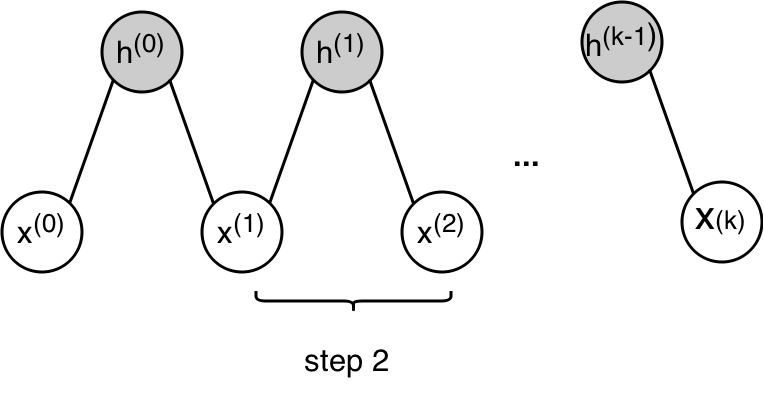
\includegraphics[width=\textwidth]{markov_chain2.png}}
% 		\end{columns}
% 		}
% 		\only<3->{
% 		\begin{columns}[c]
% 			  \column{1.5in}
% 
% 			  \column{1.5in}
% 			  \framebox{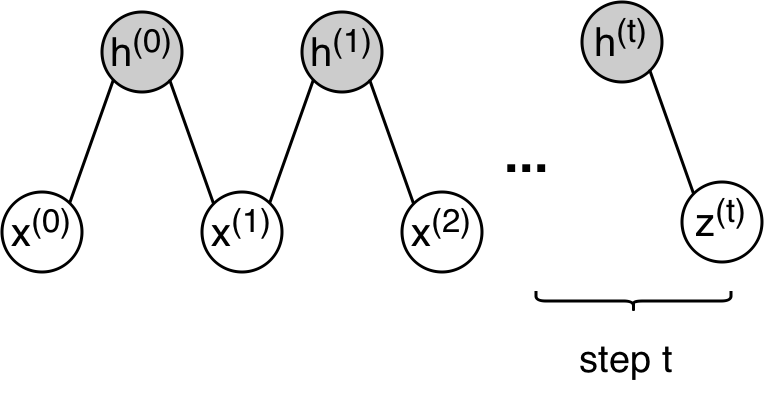
\includegraphics[width=\textwidth]{markov_chaint.png}}
% 		\end{columns}
% 		}
% 		
% 	\only<4->{$t=1$, Gibbs step $\rightarrow$ \textcolor{red}{Constrastive Divergence}}
	\end{frame}
	
	\begin{frame}[t]{Contrastive Divergence}
% 	 \textcolor{blue}{Constrastive Divergence}\\
	 \begin{itemize}
	    \item Performing k-Gibbs steps to generate $P_k(\x|\btheta)$, approximation of model distribution
	    
	    \item Difference between approximation and true model distribution:
		\begin{align}
		    KL(P_{k}(\x|\btheta)\|P(\x|\btheta))\nonumber
		\end{align}
	    \item Constrastive Divergence (CD):
	    \begin{align}
	    KL(Q(\x)\|P(\x|\btheta))- KL(P_{k}(\x|\btheta)\|P(\x|\btheta))\nonumber
	    \end{align}
	    
	    \item With enough steps the Markov chain converges to stationary distribution:
		  \begin{align}
		      P_{k\rightarrow \infty}(\x|\btheta)=P(\x|\btheta)\nonumber
		  \end{align}
	    \item CD-1 performs well in practice
	 \end{itemize}
	  
	 
	\end{frame}
	
	\begin{frame}[t]{Constrasive Divergence}
	 \txtcolb{Parameter Update}
	 \begin{align}
	  \mathrm{min} KL(Q(\x)|P(\x|\btheta)) \sim \mathrm{min} \log P(\x|\btheta)\nonumber\\
	  
	 \end{align}

	 \begin{align}
	  \Delta \btheta \sim KL(P(\x|\btheta)\|P_{k}(\x|\btheta))\nonumber
	 \end{align}

	\end{frame}





  
%% =========
% \section{Multilayer Neural Network}%4 folies
% 	\subsection{Function and Training}		
% 	\begin{frame}[t]{Structure and Function}
% 	\txtcolb{N-hidden layers neural network }
% 	  \begin{minipage}{0.45\linewidth}
% 	      \begin{itemize}
% 	       \itemsep10pt
% 	       \item Hidden layer pre-activation:\\
% 	       $\mathbf{a}(\x) =\mathbf{W}^{(1)}\x + \mathbf{b}^{(1)}$\\
% 	       $a_{j}(\x) = \sum_i w_{ji}^{(1)}x_{i} + b_{j}^{(1)}$
% 	       \item Hidden layer activation:\\
% 	       $\h = f(\mathbf{a})$
% 	       \item Output layer activation:\\
% 	       $\hat{y}(\x) = o(\mathbf{W}^{(N+1)}\h^{(N)} + \mathbf{b}^{(N+1)} )$
% 	      \end{itemize}
% 	  \end{minipage}
% 	  
% % 	  \begin{minipage}{0.45\linewidth}
% % 		\begin{figure}
% % 		      \includegraphics{}
% % 		\end{figure}
% % 	  \end{minipage}
% 
% 	\end{frame}
% 	
% 	\begin{frame}[t]{Training}
% 		\textcolor{blue}{\Large Empirical Risk Minimization}
% 		\begin{itemize}
% 		 \item learning algorithms\\
% 		 \begin{eqnarray}
% 			\text{arg}~\underset{\btheta}{\mathrm{min}} \frac{1}{M}\sum_m l(\hat{y}(\x^{(m)};\btheta),y^{(m)}) + \lambda \Omega(\btheta)\nonumber
% 			\end{eqnarray}
% 		 \item loss function $l(\hat{y}(\x^{(m)};\btheta),y^{(m)})$ \\
% 			for sigmoid activation $l(\btheta)= \sum_m \frac{1}{2} \left\| y^{(m)}-\hat{y}^{(m)}\right\| ^2$\\
% 		 \item regularizer $\lambda \Omega(\btheta)$
% 		\end{itemize}
% 		
% 		\txtcolb{Optimization}
% 		\begin{itemize}
% 		 \item Gradient calculation with Backpropagation
% 		 \item Stochastic/Mini-batch gradient descent
% 		\end{itemize}
% 
% 		
% 		
% 	\end{frame}
% 	
% 	
% 	\subsection{Problems and Solutions}
% 		
% 	\begin{frame}[t]{Pre-training}
% 		\begin{minipage}[h]{\linewidth}
% 		\txtcolb{Vanishing Gradient}
% 			\begin{itemize}
% 				\item Training time increases as network gets deeper
% 				\item Gradient shrink exponentially and training end up local minima
% 				\item Caused by random initialization of network parameters
% 			\end{itemize}
% 		\end{minipage}\vspace{5mm}
% 		\begin{minipage}[h]{\linewidth}
% 		\only<1-1>{
% 		\begin{figure}
% 		 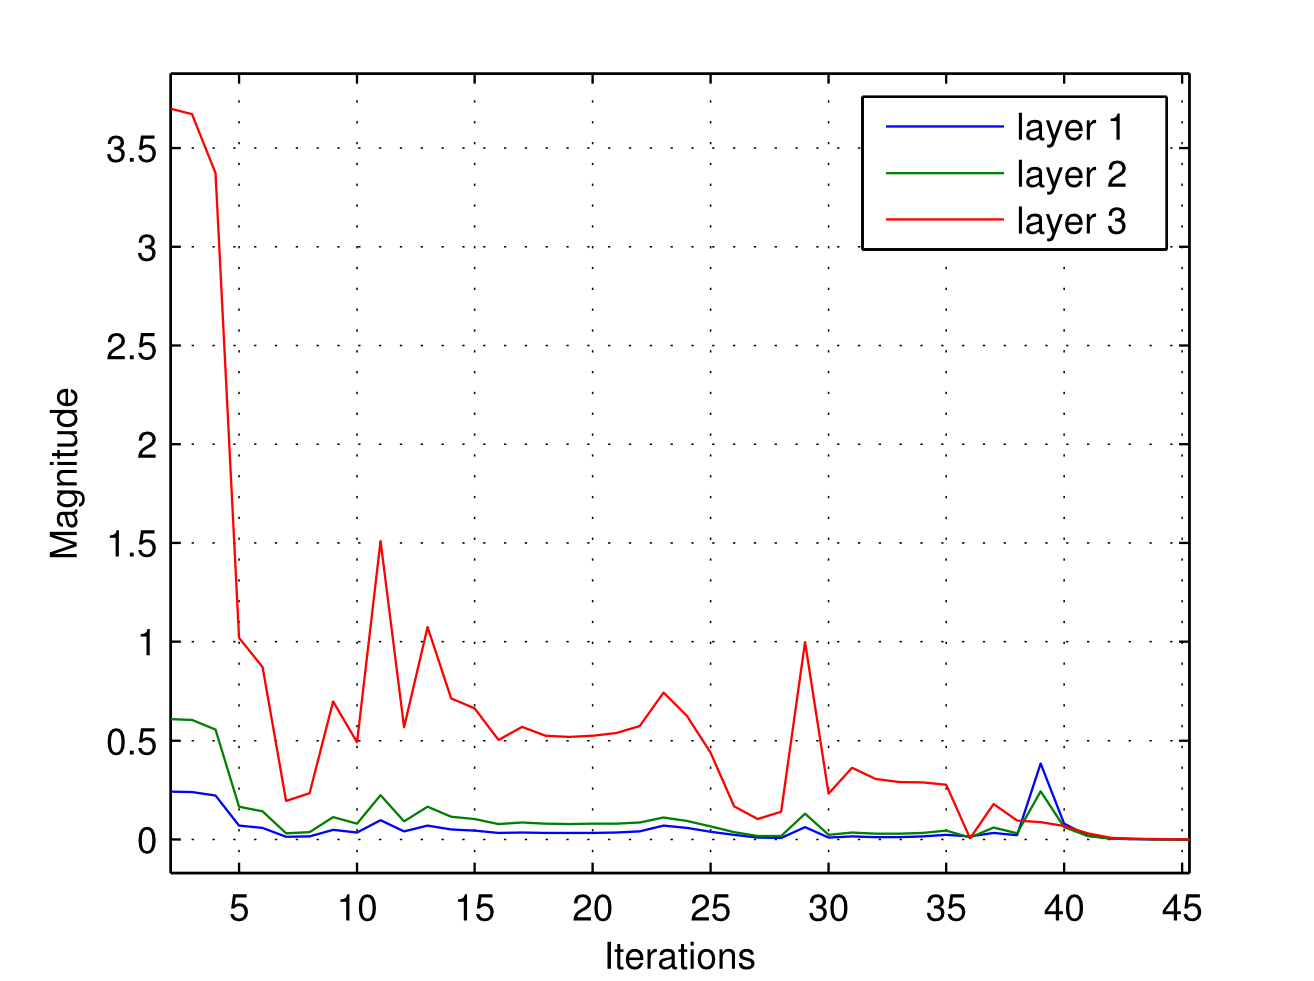
\includegraphics[width=0.6\textwidth]{GradVanishing.png}
% 		\end{figure}
% 
% 		}
% 		\visible<2->{
% 		\txtcolb{Unsupervised layerwise pre-training}
% 		\begin{itemize}
% 		 \itemsep8pt
% 		 \item Pretrain the deep network layer by layer to build a stacked auto-encoder
% 		 \item Each layer is trained as a single hidden layer auto-encoder by minimizing average reconstruction error:\\
% 		      $\mathrm{min}~l_{AE} = \sum_m \frac{1}{2}\left\|\x^{(m)}-\hat{\x}^{(m)}\right\|^2$
% 		 \item Fine-tuning the entire deep network with supervised training
% 		\end{itemize}
% 		}
% 		\end{minipage}		
% 	\end{frame}
% 
% % 		\begin{itemize}
% % 			\item Optimization problem non-convex\\
% % 			$\Rightarrow$ getting stuck in poor local minima
% % 			\item Diffusion of gradients
% % 			\item Large p small n problem $\Rightarrow$ overfitting
% % 	
% % 	\end{itemize}
% %%%%%%%%%%%%%%%%%%%%%%%%%Noob pictures for pretraining%%%%%%%%%%%%%%%
% 	\begin{frame}[t]{Pre-training}
% 	 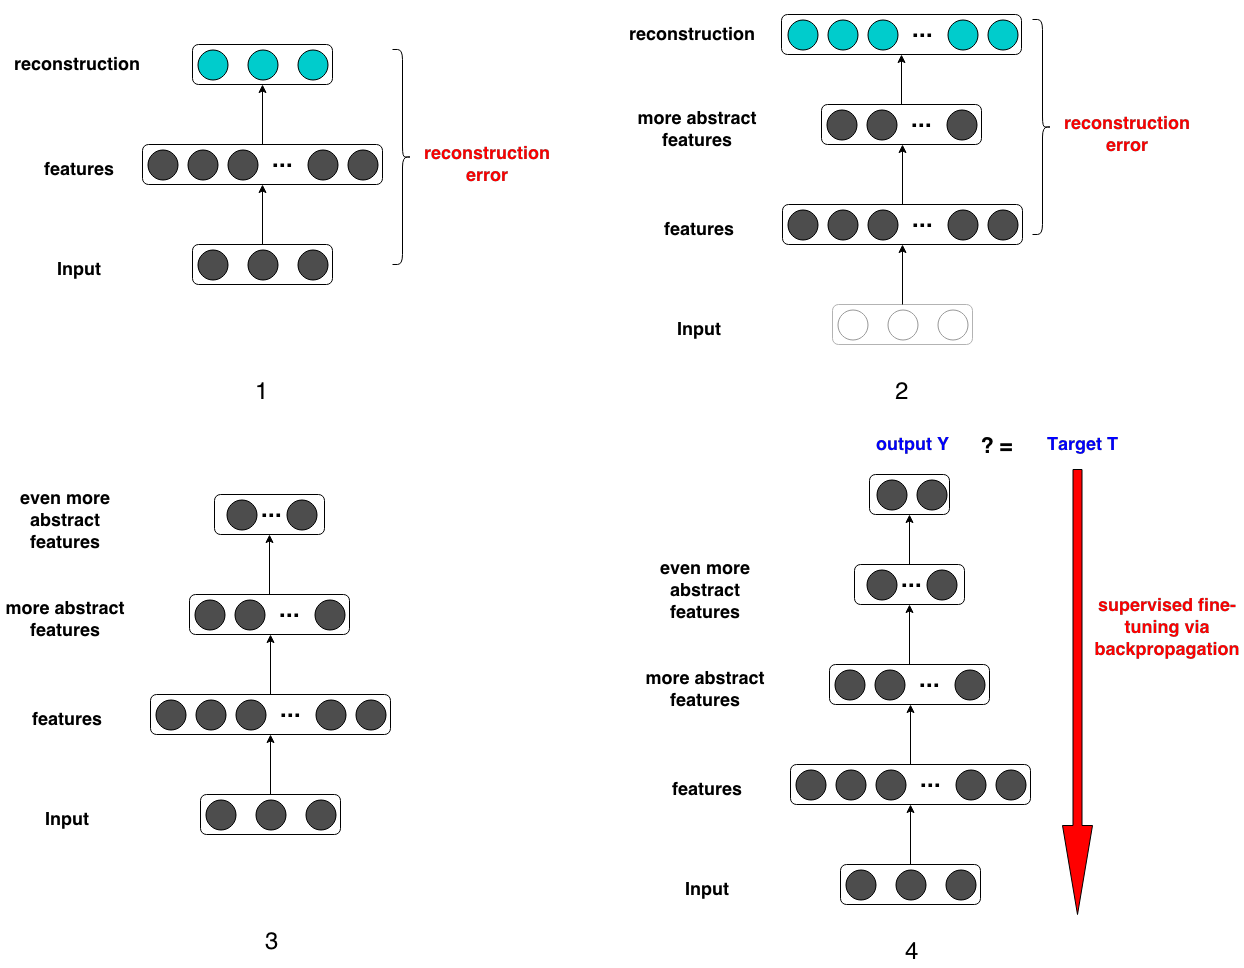
\includegraphics[width=0.9\linewidth]{layerwisewhole.png}
% 	\end{frame}
% 
% %%%%%%%%%%%%%%%%%%%%%%%%%
% 
% 	
% 	\begin{frame}[t]{Regularization}
% 		\begin{minipage}[h]{\linewidth}
% 		\txtcolb{Overfitting}
% 			\begin{itemize}
% 				\item Huge amount of parameters in deep network
% 				\item Not enough data for training
% 				\item Poor generalization 
% 			\end{itemize}
% 		\end{minipage}\vspace{5mm}
% 		\visible<2->{
% 		\begin{minipage}[h]{\linewidth}
% 		\txtcolb{Regularization}
% 			\begin{itemize}
% 			\item Add weight penalization $\lambda \left\| \mathbf{w} \right\| _{p}$ to loss function 
% 			      \begin{eqnarray}
% 			      \text{arg}~\underset{\btheta}{\mathrm{min}} \frac{1}{M}\sum_m l(\hat{y}(\x^{(m)};\btheta),y^{(m)}) + \lambda \left\| \mathbf{w} \right\| _{p}\nonumber
% 			      \end{eqnarray}
% 			\item 	In convex optimization:
% 	 		\begin{eqnarray}
% 			\text{arg}~\underset{\btheta}{\mathrm{min}} \frac{1}{M}\sum_m l(\hat{y}(\x^{(m)};\btheta),y^{(m)}),  s.t. \left\|\mathbf{w}\right\|_p \leq C\nonumber
% 			\end{eqnarray}
% 			\end{itemize}
% 		\end{minipage}	
% 		}
% 	\end{frame}
% 	
% 	\begin{frame}[t]{Regularization}
% 	\txtcolb{P-Norm}
% 	\begin{eqnarray}
% 			      \left\| \mathbf{w} \right\| _{p} := \left( \sum_{n=1}^{n} |w_{i}|^{p} \right) ^{1/p} = \sqrt[p]{|w_1|^p +,..., +|w_n|^p}\nonumber
% 	\end{eqnarray}
% 	Widely used: L1- and L2-regularization ($p=1$ and $p=2$)
% 	\begin{figure}[t]
% 	\includegraphics<1>[width=0.7\linewidth]{contoursreg.png}
% 	\includegraphics<2>[width=0.7\linewidth]{l1vsl2.png}
% % 	 \only<1-1>{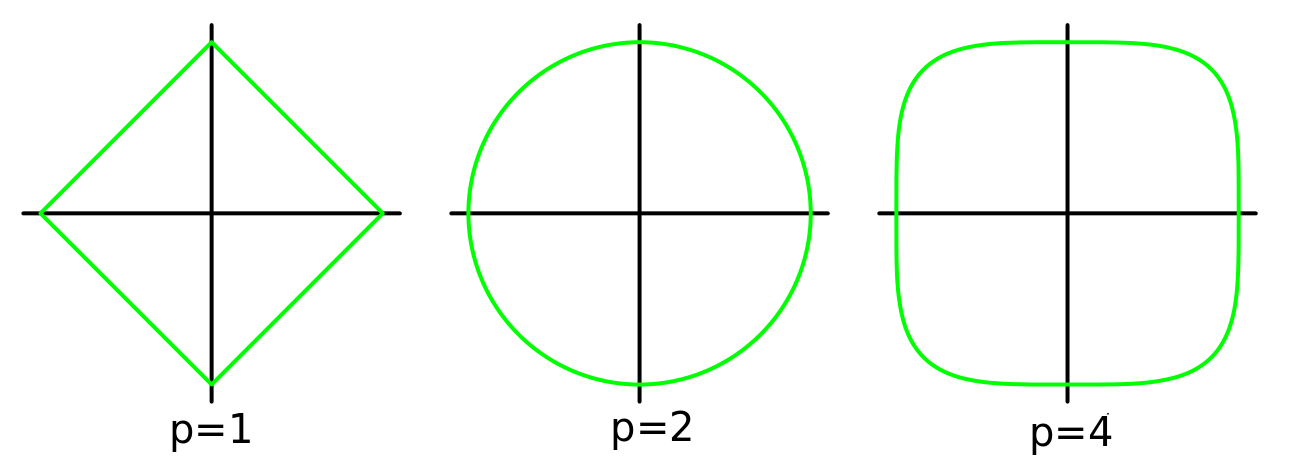
\includegraphics[width=0.7\linewidth]{contoursreg.png}}
% % 	 \only<2->{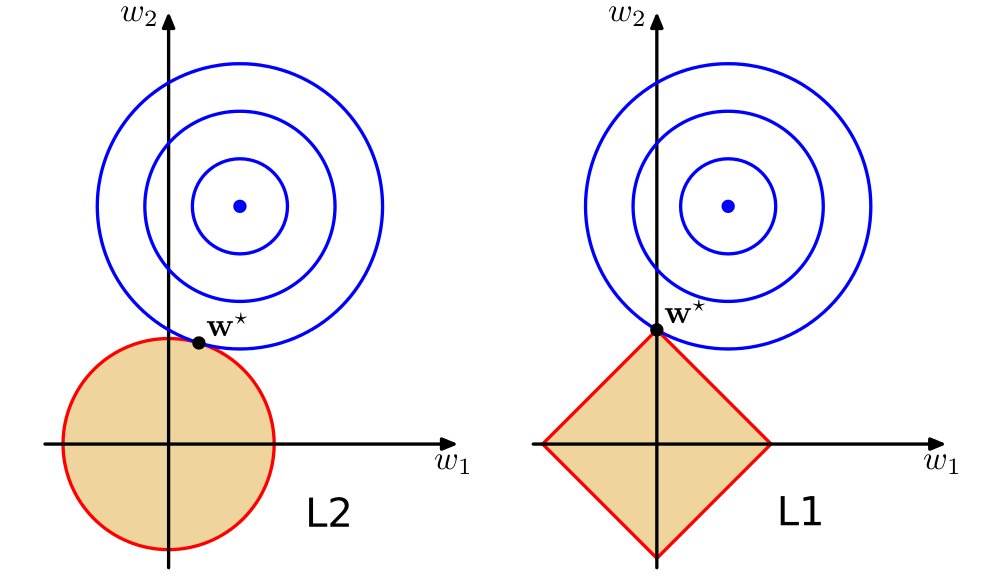
\includegraphics[width=0.7\linewidth]{l1vsl2.png}}
% 	\end{figure}
% 
% 	\end{frame}


% \section{Long Short Term Memory}
% 	\subsection{Recurrent Neural Network}
% 		\begin{frame}[t]{Recurrent Neural Network}
% % 			\begin{minipage}[t][][t]{0.48\linewidth}
% 			\textcolor{blue}{\Large Concepts of RNN}
% 				\begin{itemize}[<+->]
% % 				 \itemsep10pt
% 				 \item modelling sequential data, emotion in speech .
% 				 \item Same Structure as MLP but differs from feed-forward network, enabling
% nonlinear mapping
% 				 \only<2-2>{
% 					\begin{eqnarray}
% 						&h_{t} = \mathcal{H}(W_{xh}x_{t}+W_{hh}h_{t-1} + b_{h})\nonumber\\
% 						&y_{t} = W_{hy}h_{t} + b_{y}\nonumber
% 					\end{eqnarray}
% 				 }
% 				
% 				 \item Feedback connection between previous hidden units and current hidden units, enabling
% memory past hidden state.
% 				 \item Potentially to model arbitary dynamic system.
% 				 \item Trained with \textbf{b}ack\textbf{p}ropagation \textbf{t}hrough \textbf{t}ime (BPTT)
% 				 \note{natural extension of BP in FF network}
% 				\end{itemize}
% % 			\end{minipage}
% \vspace{5mm}
% % 		\only<1>{\begin{figure}
% % 		          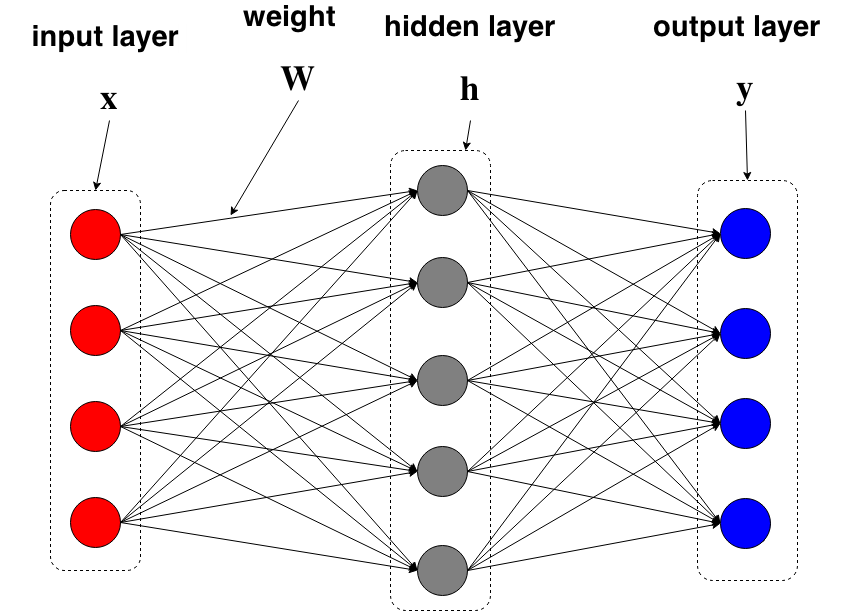
\includegraphics[width=0.5\textwidth]{NeuralNetwork.png}
% % 		         \end{figure}
% % 
% % 		}
% 		\end{frame}
% 		
% 		\begin{frame}[t]{Recurrent Neural Network}
% % 			\begin{minipage}[t][][t]{0.48\linewidth}
% 			\textcolor{blue}{\Large Concepts of RNN}
% 			\begin{minipage}[t]{0.48\linewidth}
% 				\only<1>{
% 				\begin{figure}[t]
% 				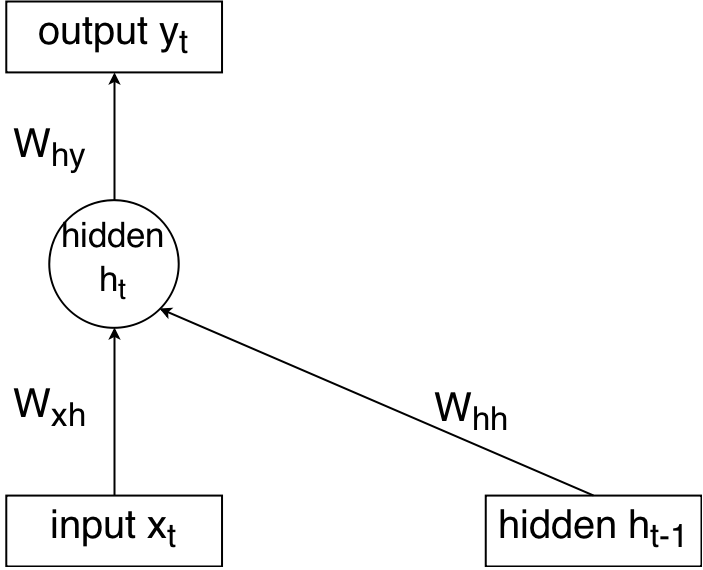
\includegraphics[width=0.8\textwidth]{RNNunit.png}
% 				\end{figure}
% 				}
% 			\end{minipage}\hfill
% 			\begin{minipage}[t]{0.48\linewidth}
% 				\only<1>{
% 				\begin{figure}[t]
% 				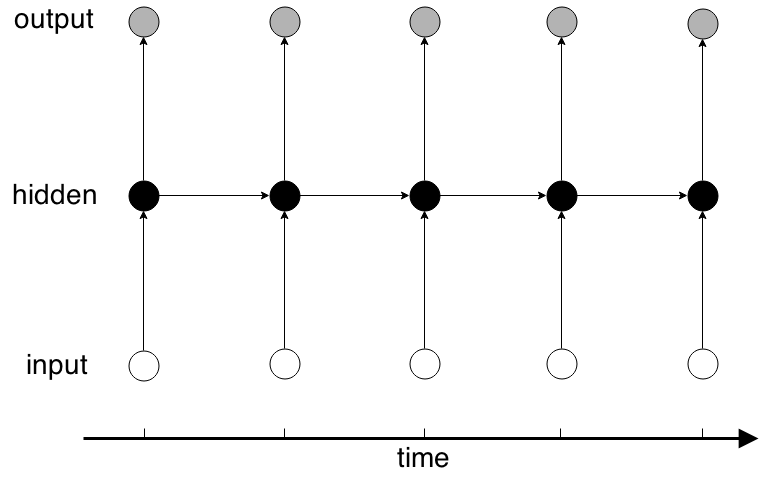
\includegraphics[width=\textwidth]{RNNStruct.png}
% 				\end{figure}
% 				}
% 			\end{minipage}
% 
% 		\end{frame}
% 		
% 		\begin{frame}[t]{From RNN to LSTM}
% 		\textcolor{blue}{\Large Problems with RNN}
% 			\begin{itemize}%[<+->]
% 			 \item gradient vanishing during backpropagation as time steps increases (>100)
% 			 \item difficult to capture long-time dependency (which is required in emotion recognition)
% 			\end{itemize}
% 		\textcolor{red}{\Large Solutions}	
% 			\begin{itemize}
% 			 \item 
% 			\end{itemize}
%     
%     
% 		\end{frame}
% 		\begin{frame}{Long short term memory}
% 		\only<1>{S. Hochreiter and J. Schmidhuber, Lovol. 9, pp. 1735-1780, 1997.}
% 		\uncover<2->{
% 		\textcolor{blue}{\Large LSTM unit}\\
% 		\begin{minipage}{0.4\linewidth}
% 			\begin{figure}
% 			 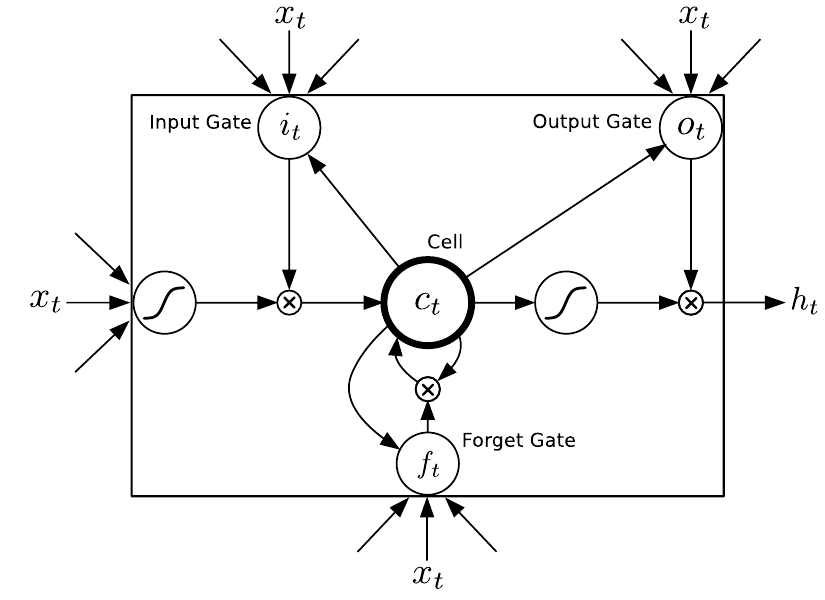
\includegraphics[width=\linewidth]{LSTMstruct.png}
% 			\end{figure}
% 		\end{minipage}
% 		\begin{minipage}[t]{0.55\linewidth}
% 			\begin{figure}
% 			 \begin{eqnarray}
% 				  i_{t} &=& \sigma (W_{xi}x_{t} + W_{hi}h_{t-1} + W_{ci}c_{t-1} +b_{i})\nonumber\\
% 				  f_{t} &=& \sigma (W_{xf}x_{t} + W_{hf}h_{t-1} + W_{cf}c_{t-1} +b_{f})\nonumber\\
% 				  c_{t} &=& f_{t}c_{t-1} + i_{t}\mathrm{tanh}(W_{xc}x_{t} + W_{hc}h_{t-1} + b_{c})\nonumber\\
% 				  o_{t} &=& \sigma (W_{xo}x_{t} + W_{ho}h_{t-1} + W_{co}c_{t} +b_{o})\nonumber\\
% 				  h_{t} &=& o_{t}\mathrm{tanh} (c_{t})\nonumber
% 			 \end{eqnarray}
% 			\end{figure}
% 		\end{minipage}
% 
% 		}
% 		\end{frame}
% 		
% 		\begin{frame}[t]{Long short term memory}
% 		\textcolor{blue}{\Large Features in LSTM}
% 		 \begin{itemize}
% 		  \item gates are trained to learn when it shoud be open/closed. 
% 		  \item Constant Error Carousel
% 		  \item preserve long-time dependency by maintaining gradient over time. 
% 		 \end{itemize}
% 		 \begin{figure}
% 		  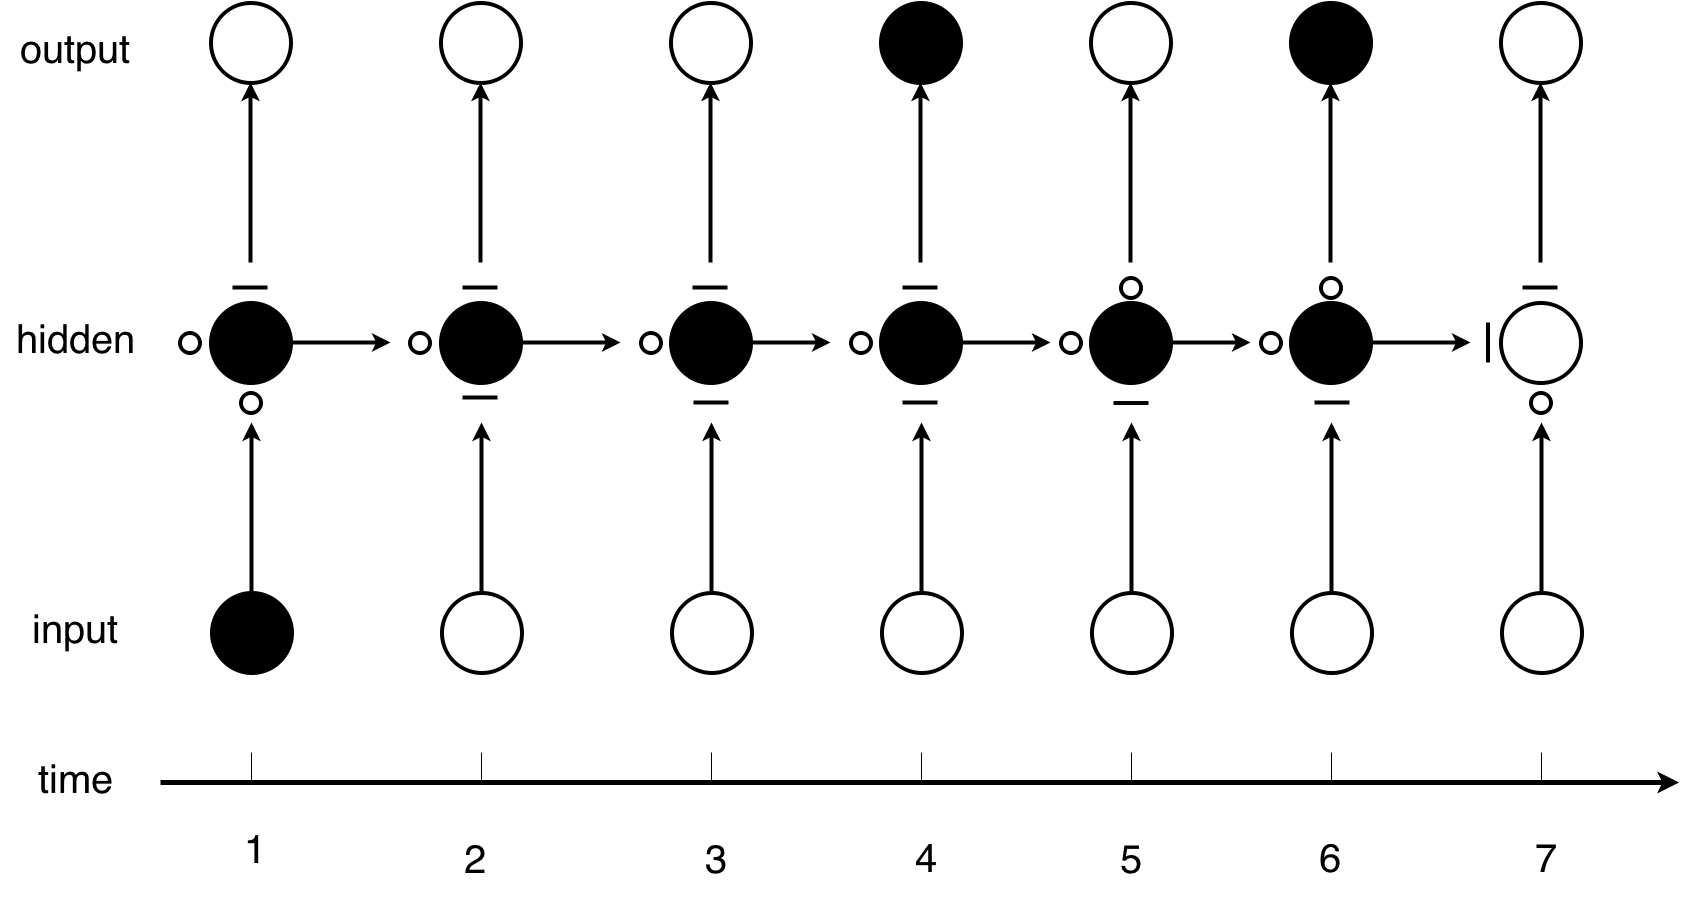
\includegraphics[width=\textwidth]{LSTMGra.png}
% 		 \end{figure}
% 
% 
% 		\end{frame}

% \section{Experiments}
% 	\begin{frame}[t]{Experiment Setup}
% 	\begin{minipage}[t]{\linewidth}
% 	 \begin{itemize}[<+->]
% 	  \item<only@1> CRBM-DNN 
% 	  \item<only@2> CRBM-LSTM
% 	  \item<only@3> LSTM
% 	  \item<only@4> LSTM with rectifier units
% 	\end{itemize}
% 	\end{minipage}\hspace{5mm}
% 	
% 	\begin{minipage}[t]{\linewidth}
% 	    \begin{figure}[b]
% 	    \only<1>{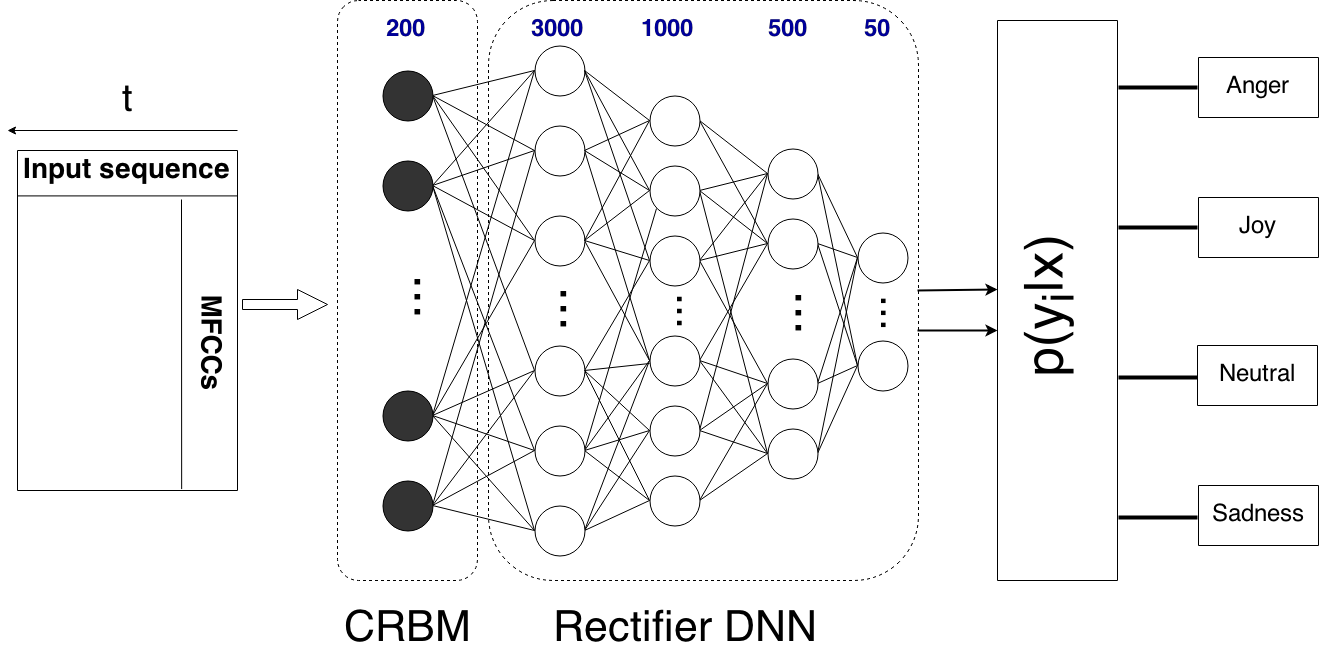
\includegraphics[width=\linewidth]{CRBMDNN.png}}
% 	    \only<2>{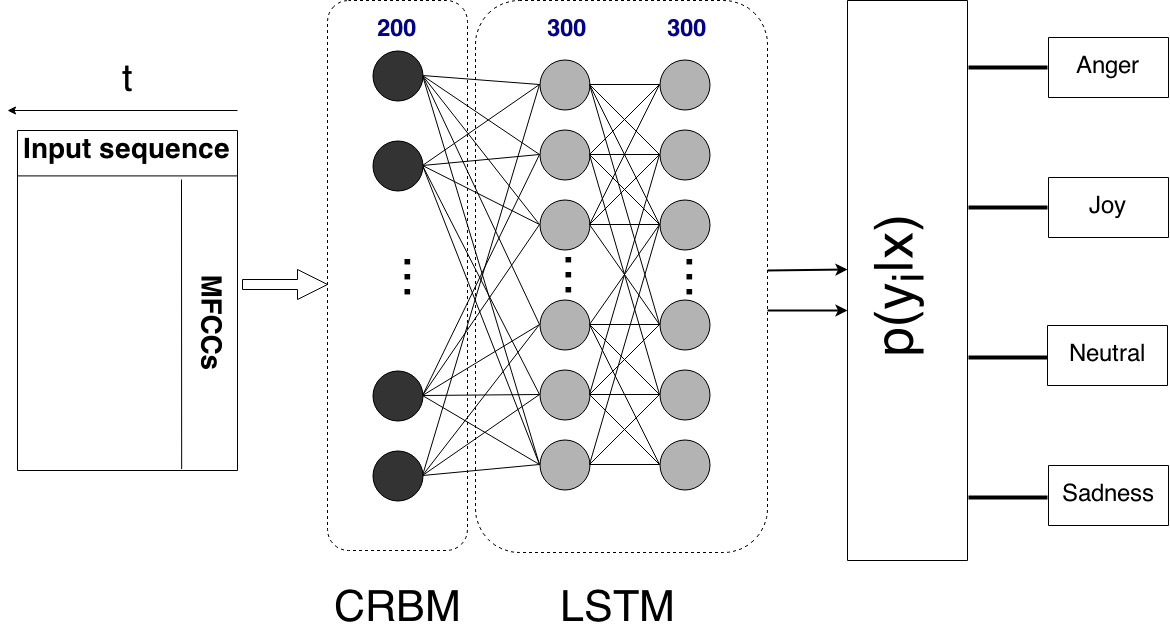
\includegraphics[width=.8\linewidth]{CRBMLSTM.png}}
% 	    \only<3>{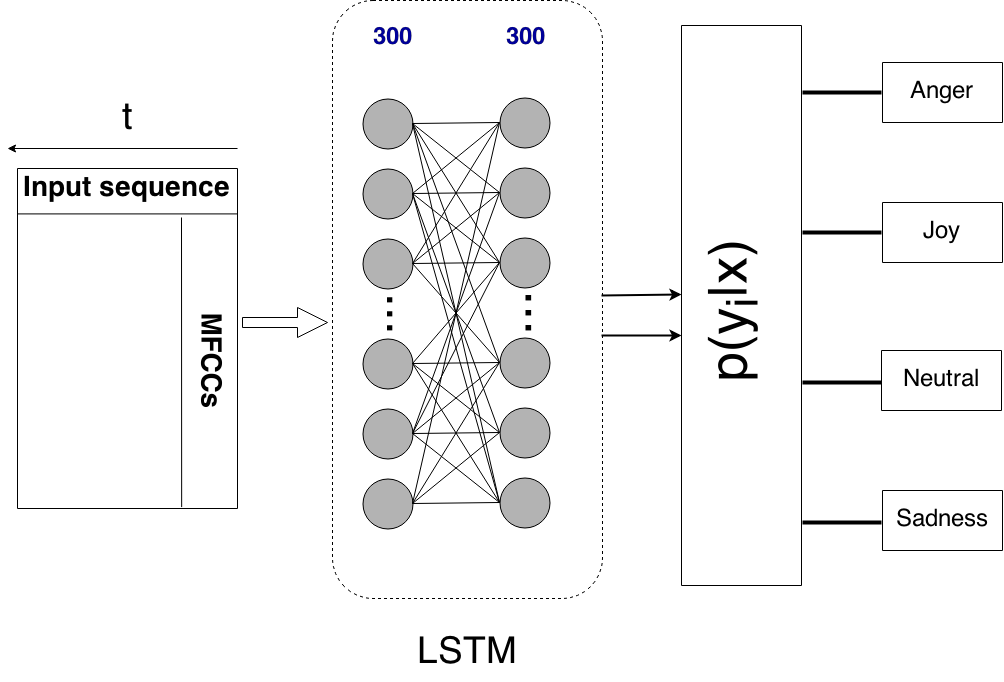
\includegraphics[width=.8\linewidth]{LSTMpure.png}}
% 	    \only<4>{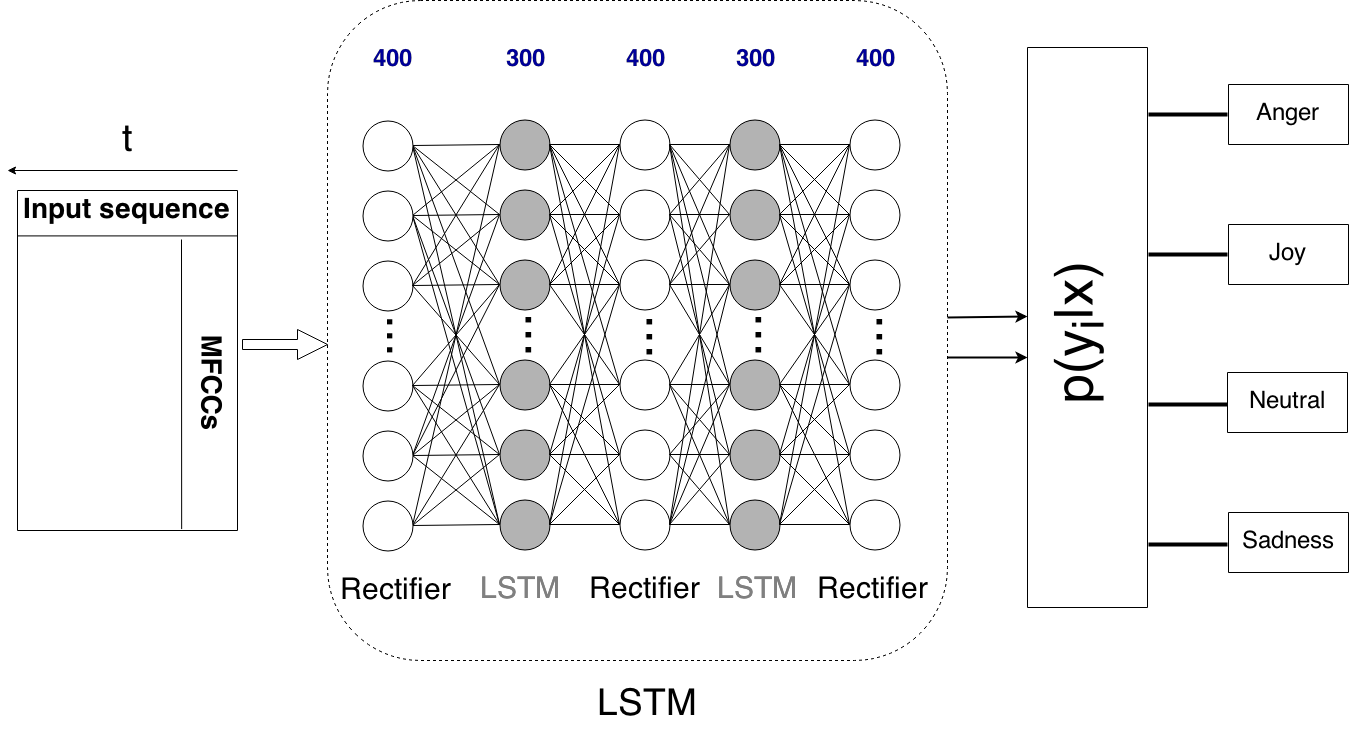
\includegraphics[width=.8\linewidth]{LSTM.png}}
% 	  \end{figure}
% 	\end{minipage}
% 
% 	\end{frame}
% 	
% 	\begin{frame}[t]{Result}
% 	      \only<1>
% 	      {
% 	      \begin{table}[htbp]\centering
% 		  \centering
% 		  Confusion matrix of CRBM-DNN result
% 		  \vspace{10mm}
% 		  \begin{tabular*}{\linewidth}{@{\extracolsep{\fill}} cl*{4}c @{}}
% 		      \toprule
% 		      & \multicolumn{5}{c}{\textit{{Classfied}}} \\[1ex]
% 		  %     \midrule
% 		      \multirow{5}{*}{\textit{True}}
% 		      & & Joy & Neutral & Sadness & Anger \\
% 		  %     \cmidrule{2-12}
% 		      & Joy             &\textcolor{red}{57.7\%} &1.4\%   		  & 0.0\%		& 40.8\%\\
% 		      & Neutral         & 17.7\%			&\textcolor{red}{54.4\%} &25.3\%   	&2.5\%     \\
% 		  %     \rot{\rlap{~\textit{{True}}}}
% 		      & Sadness         &1.6\%			&27.9\%   		  &\textcolor{red}{70.5\%}   &0.0\%    \\
% 		      & Anger           & 39.4\%			&1.6\%  		  &0.0\%   	&\textcolor{red}{59.1\%}    \\
% 		      \midrule
% 		      & \multicolumn{5}{c}{recognition rate:59.76\%}\\
% 		      \bottomrule
% 		  %     \cmidrule[1pt]{2-12}
% 		    \end{tabular*}
% 		  \label{tab:CRBMDNN}
% 	      \end{table}
% 	      }
% 	      \only<2>
% 	      {
% 		\begin{table}[htbp]\centering
% 		\centering
% 		Confusion matrix of CRBM-LSTM result
% 		\vspace{10mm}
% 		\begin{tabular*}{\linewidth}{@{\extracolsep{\fill}} cl*{4}c @{}}
% 		    \toprule
% 		    & \multicolumn{5}{c}{\textit{{Classfied}}} \\[1ex]
% 		%     \midrule
% 		    \multirow{5}{*}{\textit{True}}
% 		    & & Joy & Neutral & Sadness & Anger \\
% 		%     \cmidrule{2-12}
% 		    & Joy             &\textcolor{red}{11.3\%} &9.9\%   		  &   2.8\%	&    76.1\%\\
% 		    & Neutral         & 0.0\%			&\textcolor{red}{72.2\%} &17.7\%   	&10.1\%     \\
% 		%     \rot{\rlap{~\textit{{True}}}}
% 		    & Sadness         &0.0\%			&4.8\%   		  &\textcolor{red}{88.7\%}   &6.5\%    \\
% 		    & Anger           & 0.8\%			&1.6\%  		  &0.0\%   	&\textcolor{red}{97.6\%}    \\
% 		    \midrule
% 		    & \multicolumn{5}{c}{recognition rate: 71.98\%}\\
% 		    \bottomrule
% 		%     \cmidrule[1pt]{2-12}
% 		  \end{tabular*}
% 		\label{tab:CRBMLSTM}
% 		\end{table}
% 	      }
% 	      \only<3>
% 	      {
% 		\begin{table}[htbp]\centering
% 		\centering
% 		Confusion matrix of pure LSTM result
% 		\vspace{10mm}
% 		\begin{tabular*}{\linewidth}{@{\extracolsep{\fill}} cl*{4}c @{}}
% 		    \toprule
% 		    & \multicolumn{5}{c}{\textit{{Classfied}}} \\[1ex]
% 		%     \midrule
% 		    \multirow{5}{*}{\textit{True}}
% 		    & & Joy & Neutral & Sadness & Anger \\
% 		%     \cmidrule{2-12}
% 		    & Joy             &\textcolor{red}{66.2\%} &4.2\%   		  &   0.0\%	&    29.6\%\\
% 		    & Neutral         &6.3\%			&\textcolor{red}{79.7\%} &10.2\%   	&3.8\%     \\
% 		%     \rot{\rlap{~\textit{{True}}}}
% 		    & Sadness         &0.0\%			&19.7\%   		  &\textcolor{red}{80.3\%}   &0.0\%    \\
% 		    & Anger           & 12.6\%			&0.8\%  		  &0.0\%   	&\textcolor{red}{86.6\%}    \\
% 		    \midrule
% 		    & \multicolumn{5}{c}{recognition rate: 81.59\%}\\
% 		    \bottomrule
% 		%     \cmidrule[1pt]{2-12}
% 		  \end{tabular*}
% 		\label{tab:pureLSTM}
% 		\end{table}
% 	      }
% 	      \only<4>
% 	      {
% 		\begin{table}[htbp]\centering
% 		\centering
% 		Confusion matrix of LSTM-Rectifier result
% 		\vspace{10mm}
% 		\begin{tabular*}{\linewidth}{@{\extracolsep{\fill}} cl*{4}c @{}}
% 		    \toprule
% 		    & \multicolumn{5}{c}{\textit{{Classfied}}} \\[1ex]
% 		%     \midrule
% 		    \multirow{5}{*}{\textit{True}}
% 		    & & Joy & Neutral & Sadness & Anger \\
% 		%     \cmidrule{2-12}
% 		    & Joy             &\textcolor{red}{57.7\%} &7.0\%   		  &   0.0\%	&    35.2\%\\
% 		    & Neutral         &6.3\%			&\textcolor{red}{86.1\%} &6.3\%   	&1.3\%     \\
% 		%     \rot{\rlap{~\textit{{True}}}}
% 		    & Sadness         &0.0\%			&6.6\%   		  &\textcolor{red}{93.4\%}   &0.0\%    \\
% 		    & Anger           & 8.7\%			&0.0\%  		  &0.0\%   	&\textcolor{red}{91.3\%}    \\
% 		    \midrule
% 		    & \multicolumn{5}{c}{recognition rate: 83.43\%}\\
% 		    \bottomrule
% 		%     \cmidrule[1pt]{2-12}
% 		  \end{tabular*}
% 		\label{tab:LSTMRec}
% 		\end{table}
% 	      }
% 	\end{frame}



\section{Conclusion and Outlook}
      \begin{frame}[t]{Conclusion}
	  \begin{itemize}
	  \itemsep10pt
	  \item Model with long-term dependencies shall be used for speech emotion
	  \item CRBM is appropriate for short-term modelling, but not for long-term variation
	  \item LSTM is good at modelling long time dependency 
	  \item Frame-based classification can also reach good result
		\vspace{5mm}
		\begin{itemize}
		 \itemsep10pt
		 \item CRBM-LSTM $71.98\%$
		 \item LSTM $81.59\%$
		 \item LSTM with rectifier layers $83.43\%$
		\end{itemize}
	  \end{itemize}
      \end{frame}
      
      \begin{frame}[t]{Outlook}
	  \begin{itemize}
	   \itemsep15pt
	   \item Stacking CRBM to form deeper structure
	   \item Train CRBM with more/larger database 
	   \item Second order optimization to speed up learning process
	   \item Bi-directional LSTM, capturing future dependencies
	  \end{itemize}

      \end{frame}

      \begin{frame}{End}
	\begin{minipage}[c]{\linewidth}
	\centering
	\textbf{\Huge Thank You!}
	\end{minipage}
      \end{frame}



\end{document}
